\chapter{Market data curation and feature construction}
\label{chap:data}

In this chapter, we will outline the details of our data collection process, and how this data can subsequently form a historical order book in order to serve as the historical data source for the match engine.
We will describe the way that raw market event data was collected from an exchange (Bittrex\footnote{https://bittrex.com/} in our case) and processed in order to form a historical limit order book.
A sample period from the data set collected will then be investigated in order to find and visualize the properties of the market in question and the behavior of the corresponding market participants.
The goal of the investigation is to find hypotheses which state why certain occurrences might be beneficial to consider for the purpose of limit order placement.
Thus, the findings serve as the basis for the feature construction process which determines the input for the learner.
Therefore, in the last section of this chapter, we will construct features which adequately address the stated hypotheses.
Finally, the features constructed will serve as the observed state that is to be evaluated by the reinforcement learning agents described in Chapter \ref{chap:setup}.

\section{Collection of market events}
\label{sec:data-collection}

In most exchanges in the cryptocurrency domain, real-time market data is freely available. 
There is often a limit as to how far into the past historical data is retained.
However, continuously recording real-time data results in a historical data set which is complete from the time when recording was started and has provided the desired data set for this research.
A historical limit order book consisting of states which store every bid and ask posted by traders is commonly referred to as a \textit{complete order book}.
The process of accumulating the data and building the order book is illustrated in a high level pipeline in Figure \ref{fig:data-pipeline} below.
\begin{figure}[H]
    \centering
    \makebox[\linewidth]{
        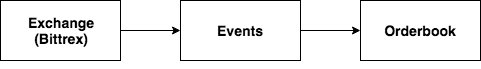
\includegraphics[width=8cm]{data-pipeline.png}
    }
    \caption{Data collection pipeline}
    \label{fig:data-pipeline}
\end{figure}
Therefore, a complete order book is being reconstructed by processing market \textit{events} that have occurred over time with a given ticker (trading pair, in our case USD/BTC).
There are three common types of events, all of which are initiated by a market participant (trader): \textit{order created}, \textit{order cancelled} or \textit{order filled} in the event that a market order crosses the spread, resulting in a trade.

Our exchange of choice for collecting data was Bittrex as this exchange provides a \textit{SignalR}\footnote{https://docs.microsoft.com/en-us/aspnet/signalr/overview/getting-started/introduction-to-signalr} (a library that abstracts \textit{HTTP} and \textit{WebSocket}) interface from which one can extract all status updates (events) from the market.
More specifically, a status update is either a buy or sell order, or a fill (e.g. trade).
Therefore, we subscribed to \texttt{https://socket.bittrex.com/signalr} and filtered the data field \texttt{M} for \texttt{updateExchangeState}.
The data type of the message contains the name of the trading pair and a nonce to identify the unique status update.
That is,
\begin{equation}
    StatusUpdate = \{name, nonce, buy_1,...buy_n, sell_1,...sell_n, fill_1,...fill_n\}
\end{equation}
, whereas $buy \in Order_{Limit}$, $sell \in Order_{Limit}$ (see Eq. \ref{eq:order-limit}) and $fill \in Trade$ (see Eq. \ref{eq:trade}).
In this regard, the orders hold an additional field $type \in \{0,1,2\}$ which specifies whether it was a \textit{create}, \textit{cancel} or \textit{change} in the order, whereby the changes of orders are neglected in our setup as this function is rarely used by traders.

It is evident that multiple events can be sent within one status update message. 
We segmented the status update into separate events with the same nonce, so that each event expressed either a limit order of a side bid or ask or a filled order resulting in a trade.
We then defined an \textit{event} as,
\begin{equation}\label{eq:event-update}
    Event = \{name, nonce, type, isTrade, trade, isBid, order\},
\end{equation}
whereas $isTrade \in \{0,1\}$ and $isBid \in \{0,1\}$ indicating whether the update contains an order or a trade. 
Finally, we made use of the data types defined in Chapter \ref{chap:preliminaries} (Sections \ref{sec:order-book} and \ref{sec:match-engine}) such that $order \in Order_{Limit}$ and $trade \in Trade$.

\section{Reconstruction of an order book with market events}
\label{sec:data-generation}

The next step was to transform the events collected into an order book structure.
By chronologically iterating over the processed events (Eq. \ref{eq:event-update}), we created a new order book state (Eq. \ref{eq:order-book-state}) for each such event.
During this iterative process, we ensured that the correct order book entries remained in future order book states, by handling the events in accordance with their respective type, as follows:
\begin{description}
    \item[Order created:] an order book entry is added to the current state.
    \item[Order cancelled:] the amount of shares as specified in the canceled order is subtracted from the entry in the current state at the corresponding price level.
    \item[Order filled:] the amount of shares traded is subtracted from the entry in the current state at the corresponding price level.
\end{description}
\hfill
\\
As a result, a \textit{list} of order book states is formed which constitutes a historical order book (Eq. \ref{eq:order-book}).
\textit{We acknowledge that a list representation is by no means the highest-performing method of implementing an order book, but for our purposes it is sufficient.}

\vfill

\section{Formulating hypotheses of the market behaviour}
\label{sec:data-hypotheses}

Let us  take a random, \textasciitilde10 minute period of the recorded market event data, and try to extract essential information from either raw events or the order book that has been generated.
Figure \ref{fig:data-price-movement} shows the price movement of the chosen sample period, indicating a movement from \$10,100 to \$10,030 and back within 10 minutes.
We first obtain an insight into the market situation with regard to some of the properties mentioned in Section \ref{sec:ob-characteristics} and understand how market participants place orders.
Our aim is then to find patterns of how market participants behave and how this may affect the market.
Subsequently, we will formulate \textit{hypotheses} which propose why certain properties might be beneficial to the order placement process, and thereby suggest which properties might be worth considering in the feature construction process. 
However, we acknowledge that the observations gleaned are based on a random sample of a historical data set,
By no means does this method guarantees that the same observations are true for any order book.

\begin{figure}[H]
    \centering
    \makebox[\linewidth]{
        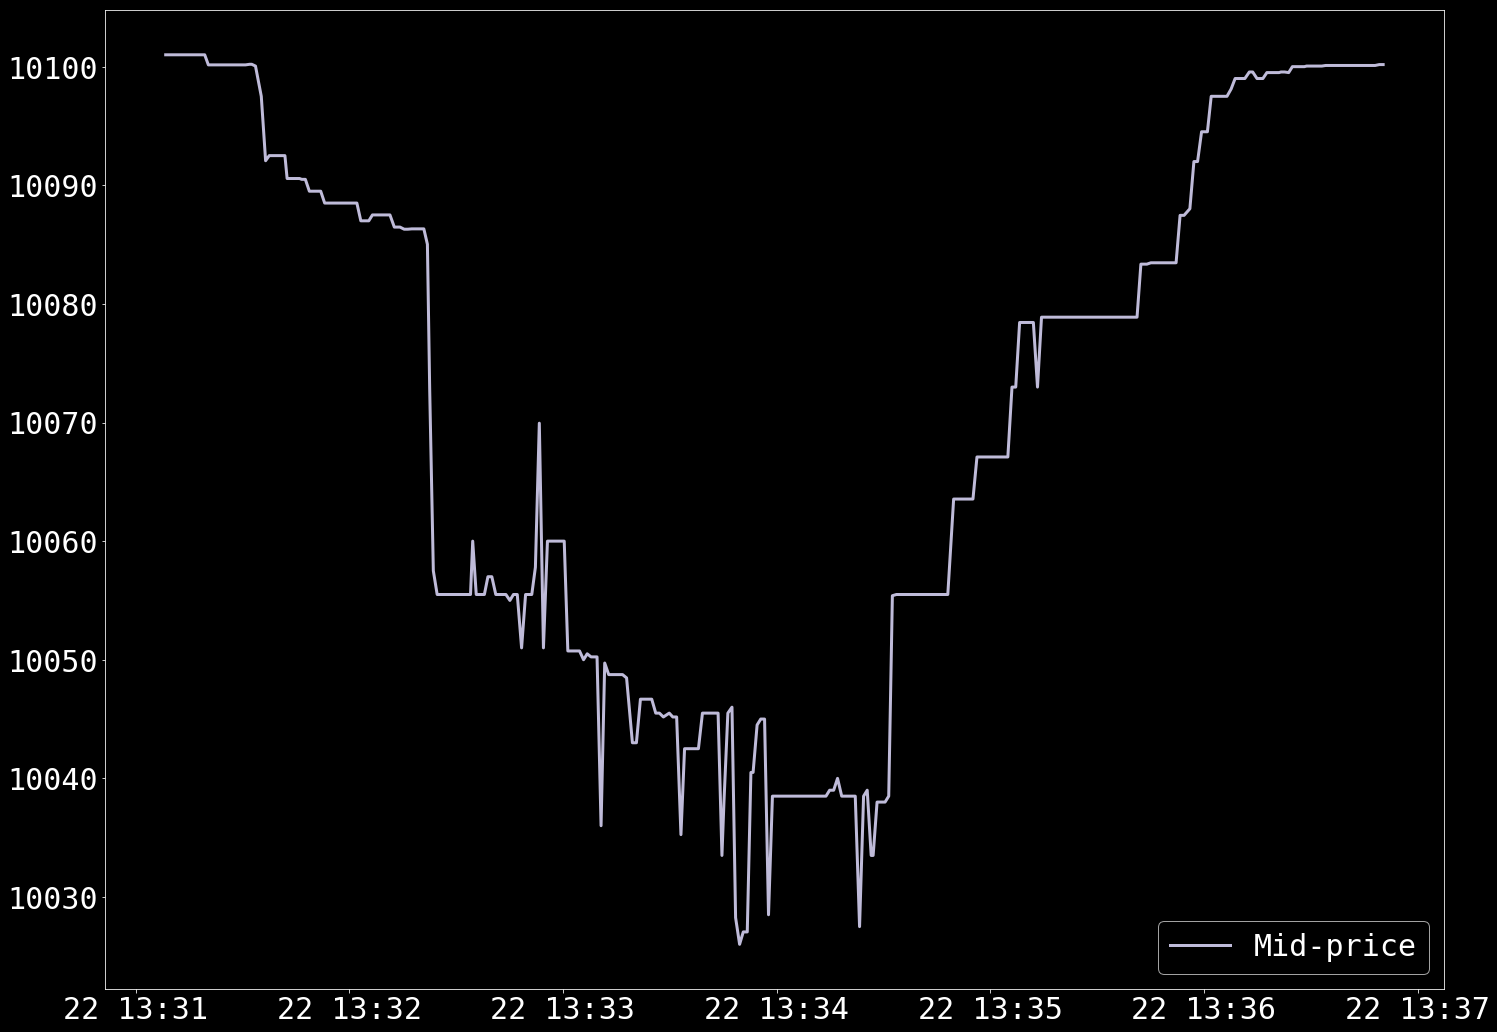
\includegraphics[width=12cm]{ob-price}
    }
    \caption{Price movement of sample data set}
    \label{fig:data-price-movement}
\end{figure}

\subsection{Importance of order prices}
\label{sec:data-hypthesis-order-price}

\begin{figure}[H]
    \centering
    \begin{subfigure}[b]{0.45\textwidth}
        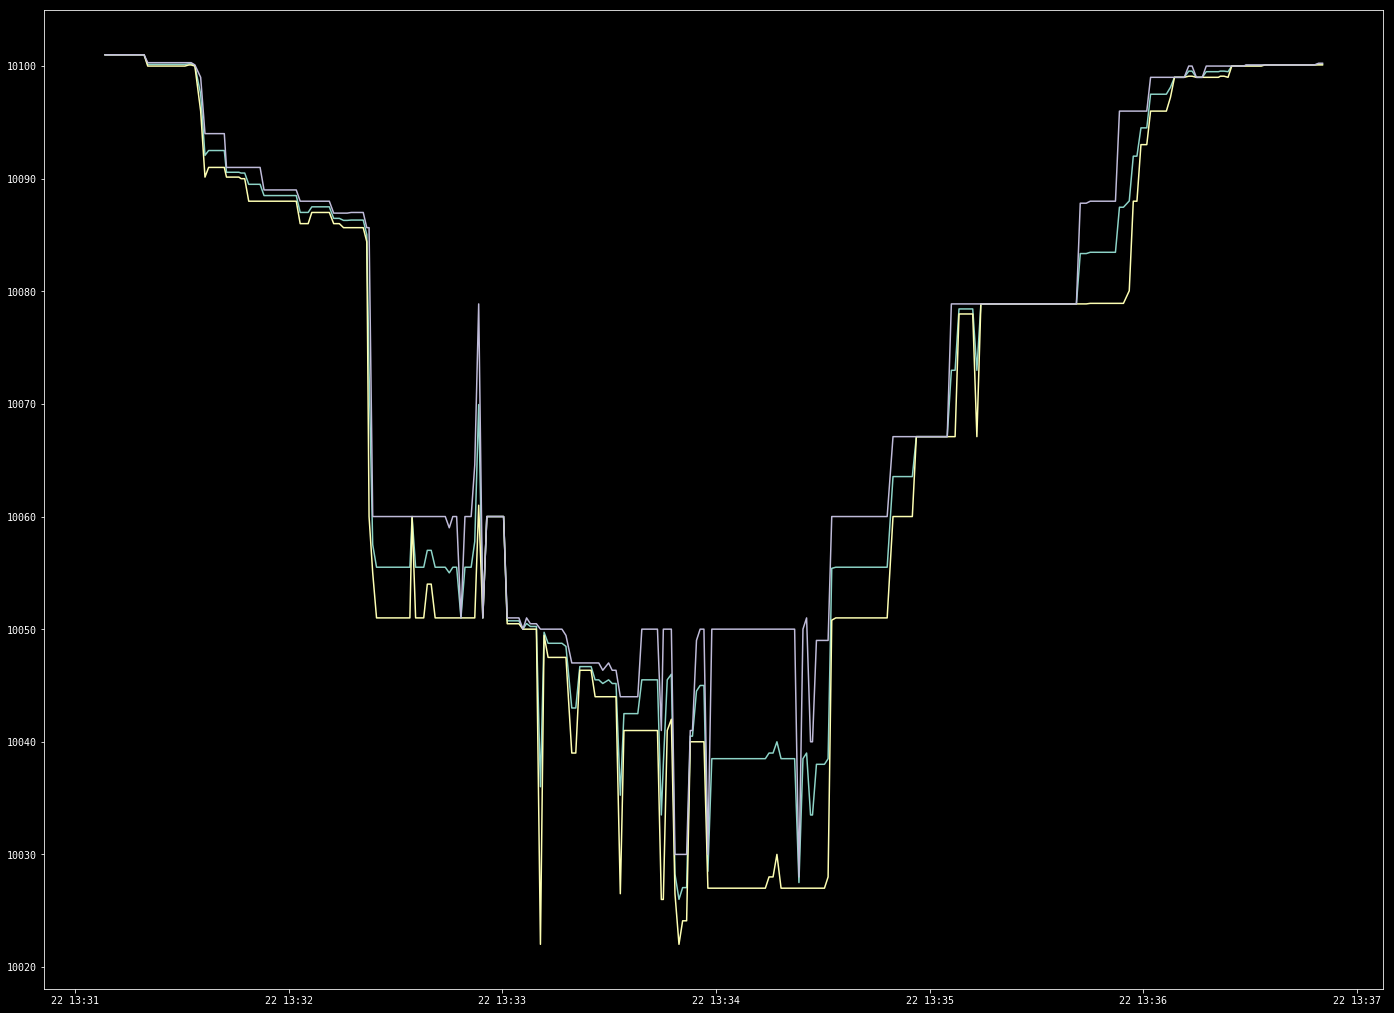
\includegraphics[width=\textwidth]{images/ob-ba-min.png}
        \caption{Best bid and best ask}
        \label{fig:ob-ba-min}
    \end{subfigure}
    ~ %add desired spacing between images, e. g. ~, \quad, \qquad, \hfill etc. 
    %(or a blank line to force the subfigure onto a new line)
    \begin{subfigure}[b]{0.45\textwidth}
        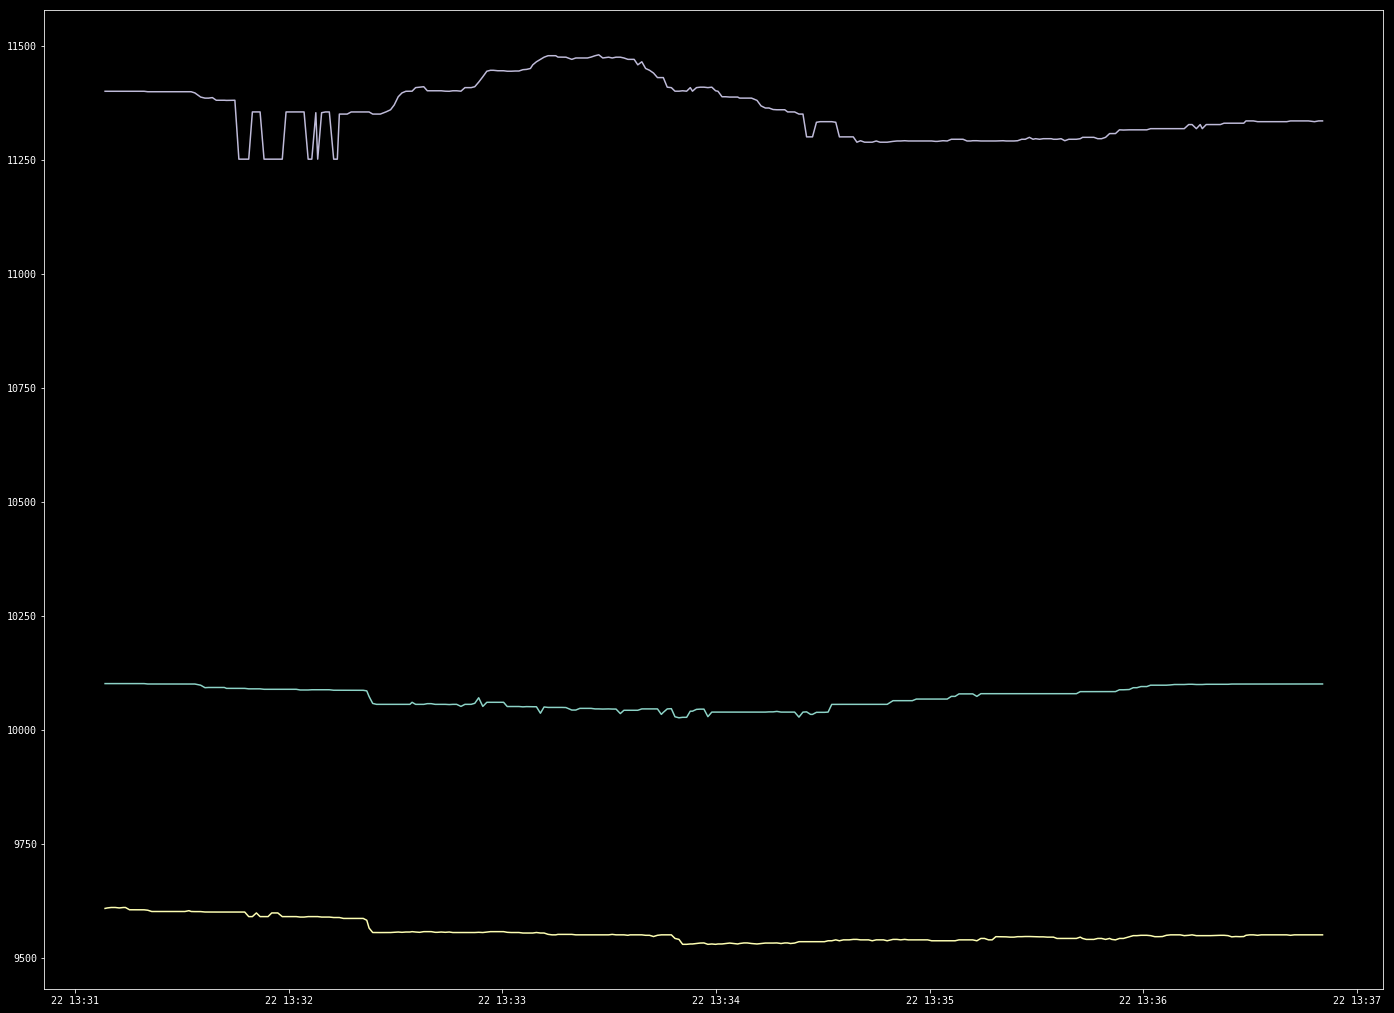
\includegraphics[width=\textwidth]{ob-ba-max}
        \caption{Deepest bid and deepest ask}
        \label{fig:ob-ba-max}
    \end{subfigure}
    \caption{USD/BTC price and bid/ask positions}\label{fig:animals}
\end{figure}

In Figure \ref{fig:ob-ba-min} we show the same price movement including the best bid and ask price.
Furthermore, the deepest level of the bid and ask ask side is shown in Figure \ref{fig:ob-ba-max}.
It is evident that the best bid and ask are close to the market price before and after the price dip, meaning the spread is narrow.
During the dip, the spread widens and is, at times, as large as \$25.
\\
\\
\textit{\textbf{Hypothesis:} participants place limit orders close to the spread when the market price is stable and place them further from the spread when the market price is fluctuating.}
\\
\\
The orders placed at the deepest level on the buyer and seller side undergo a very interesting change.
Immediately before the the price dip, ask prices start to fluctuate as some participants cancel their listings.
On the contrary, bid prices remain much more stable.
Likewise, during the fall and rise of the price, the ask price starts to increase at the deepest level of the seller side. 
This phenomenon is, at first glance, unexpected as one would expect the sell offers to decline as the price falls.
As it can be seen that the price rises shortly after the dip, we can postulate that some sellers' intentions were to incentivize buyers with the fear that sell listings could rise even further
\\
\\
\textit{\textbf{Hypothesis:} sellers incentivize buyers by placing higher prices on limit orders during a price fall.}
%\\
%\begin{figure}[H]
%    \centering
%    \begin{subfigure}[b]{0.45\textwidth}
%        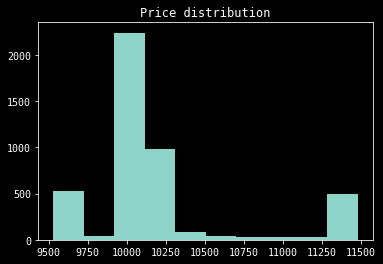
\includegraphics[width=\textwidth]{images/ob-price-bars}
%        \caption{Distribution of prices}
%        \label{fig:ob-price-dist-unfiltered}
%    \end{subfigure}
%    \begin{subfigure}[b]{0.45\textwidth}
%        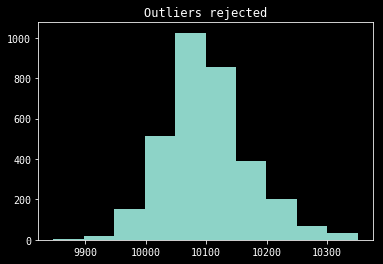
\includegraphics[width=\textwidth]{images/ob-price-bars-rejected}
%        \caption{Distribution of prices (filtered)}
%        \label{fig:ob-price-dist-filtered}
%    \end{subfigure}
%    \caption{Price distribution of events}\label{fig:price-distribution}
%\end{figure}
%
%Figure \ref{fig:ob-price-dist-unfiltered} shows the distribution of prices of all types of events (create, cancel, trade) within this data set.
%As can be seen, most of the events contain prices in the range of the traded price (see Figure \ref{fig:ob-price}) and significantly less below and above this range.
%However, the number of events increase with prices on both, the far end of the buyer and seller side, which supports the above stated hypothesis that orders deep in the book might in fact affect the price movement--even though they were not executed within the spectrum of this data set.
%We then filter events by rejecting outliers of their price $p$ according to standard deviation $\sigma$, $ |p_i - \overline{p}| < m * \sigma_{p} $, whereas $m=2$.
%As a result, Figure \ref{fig:ob-price-dist-filtered} shows the distribution of the prices from the filtered events, that follows a standard distribution.
%The mean lays at approximately \$10'100, the price level before and after the dip.
%\\
%\\
%\textit{\textbf{Hypothesis:} in case of a price dip (or raise) density estimation can be applied to find a more stable price level.}

\subsection{Importance of order volume}
\label{sec:data-hypthesis-order-volume}

It was shown that market participants position orders at different price levels as the asset price moves due to trading.
The second variable in posting orders is the volume and we aim to determine whether or not this is a factor which is affected during price movements in the given sample period.

% \begin{figure}[H]
%     \centering
%     \begin{subfigure}[b]{0.45\textwidth}
%         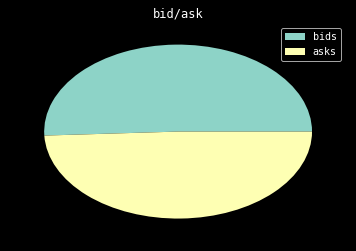
\includegraphics[width=\textwidth]{images/ob-ba-pie-all}
%         \caption{All events}
%         \label{fig:data-imbalance-events}
%     \end{subfigure}
%     \begin{subfigure}[b]{0.45\textwidth}
%         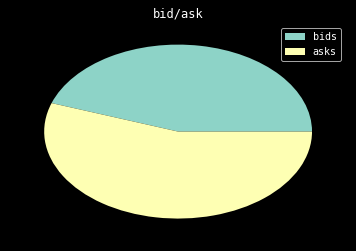
\includegraphics[width=\textwidth]{images/ob-ba-pie-trades}
%         \caption{Trades only}
%         \label{fig:data-imbalance-trades}
%     \end{subfigure}
%     \begin{subfigure}[b]{0.45\textwidth}
%         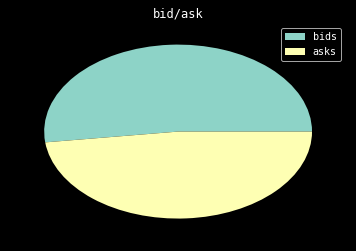
\includegraphics[width=\textwidth]{images/ob-ba-pie-created}
%         \caption{Create order only}
%         \label{fig:data-imbalance-creates}
%     \end{subfigure}
%     \begin{subfigure}[b]{0.45\textwidth}
%         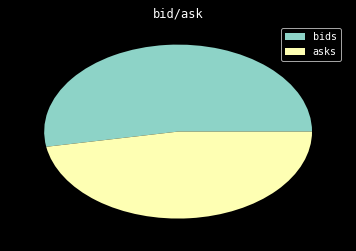
\includegraphics[width=\textwidth]{images/ob-ba-pie-cancelled}
%         \caption{Cancel orders only}
%         \label{fig:data-imbalance-cancels}
%     \end{subfigure}
%     \caption{Bid / Ask volume imbalance}\label{fig:data-imbalance}
% \end{figure}

\begin{table}[H]
\centering
\begin{tabular}{l|l|l|l|l|}
\cline{2-5}
& \textbf{All events} & \textbf{Trades only} & \textbf{Orders created} & \textbf{Orders canceled} \\ \hline
\multicolumn{1}{|l|}{\textbf{Bids}} & 51\%                & 41\%                 & 54\%                    & 57\%                      \\ \hline
\multicolumn{1}{|l|}{\textbf{Asks}} & 49\%                & 59\%                 & 46\%                    & 43\%                      \\ \hline
\end{tabular}
\caption{Bid / Ask volume imbalance}
\label{tbl:data-imbalance}
\end{table}

Table \ref{tbl:data-imbalance} shows the balance between the volumes of bid and ask orders. It does this by categorizing the events as follows: all events, trade events only, order creations, and order cancellations.
It is evident that, even though the price moved significantly within the recorded time range, all the events and trade events only (the first two categories defined above) are well balanced between the bid and ask side.
Further, it is evident that the market participants reacted to the sale of the asset by not only creating but also canceling more buy orders than sell orders.
This indicates that the market participants may have responded to the price dip by canceling their current buy orders and posting them at a lower price in the book.
Interestingly, even though the price rose after the dip, the volumes of creations and cancellations of orders on the seller side were lower.
\\
\\
\textit{\textbf{Hypothesis:} the balance (or imbalance) between volumes of bids and asks of all event types allows us to estimate the future behavior of market participants.}

\subsection{Importance of volume of orders and trades over time}
\label{sec:data-hypthesis-order-trade-volume-time}

So far, volume has been investigated as a sum of events over time.
In order to understand the behavior of participants in greater detail, a \textit{volume map} will provide an insight into single events occurring over time, as shown in the following figures.
The x-axis represents the time stamp and the y-axis is the volume of orders that were placed or resulted in trades.
For visibility reasons, the y-axis follows a log scale, since the volumes of the majority of orders and trades are small and fewer have large volumes.
Participants cannot be assigned to such orders or trades, as the trader "ID" is non-public information.
However, as we will see, one can identify some participants on the basis of their behavior.
Therefore, some of the more obvious patterns are highlighted in the figures.
\begin{figure}[H]
    \centering
    \makebox[\linewidth]{
        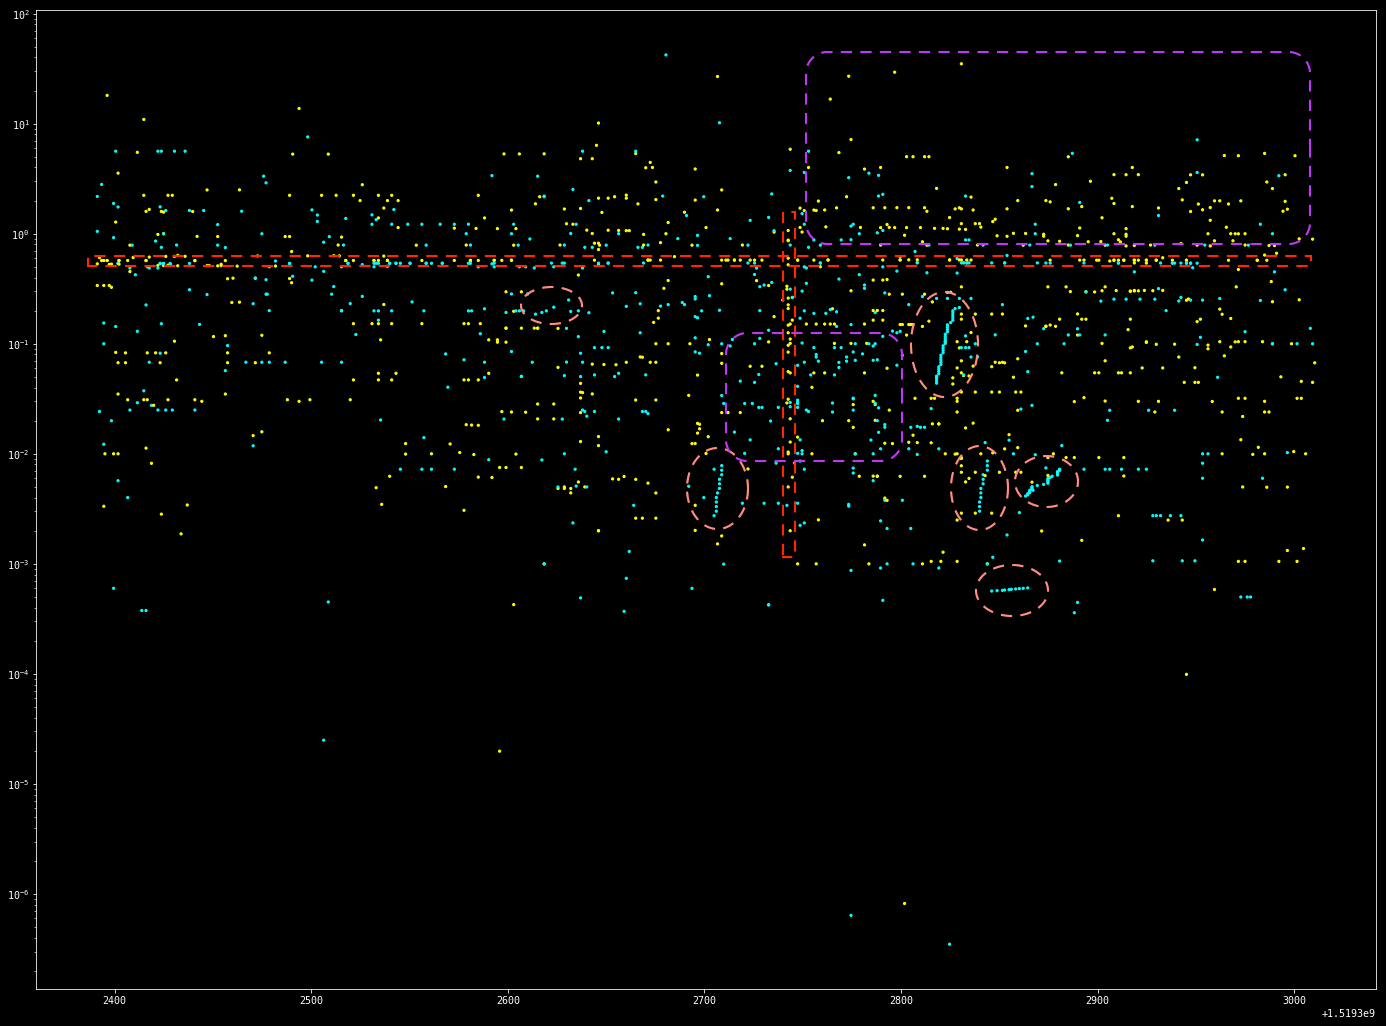
\includegraphics[width=14cm]{images/data-volmap-created}
    }
    \caption{Volume map of created bid and ask orders.}
    \label{fig:data-volmap-crated}
\end{figure}
\ref{fig:data-price-movement}).
\begin{figure}[H]
    \centering
    \makebox[\linewidth]{
        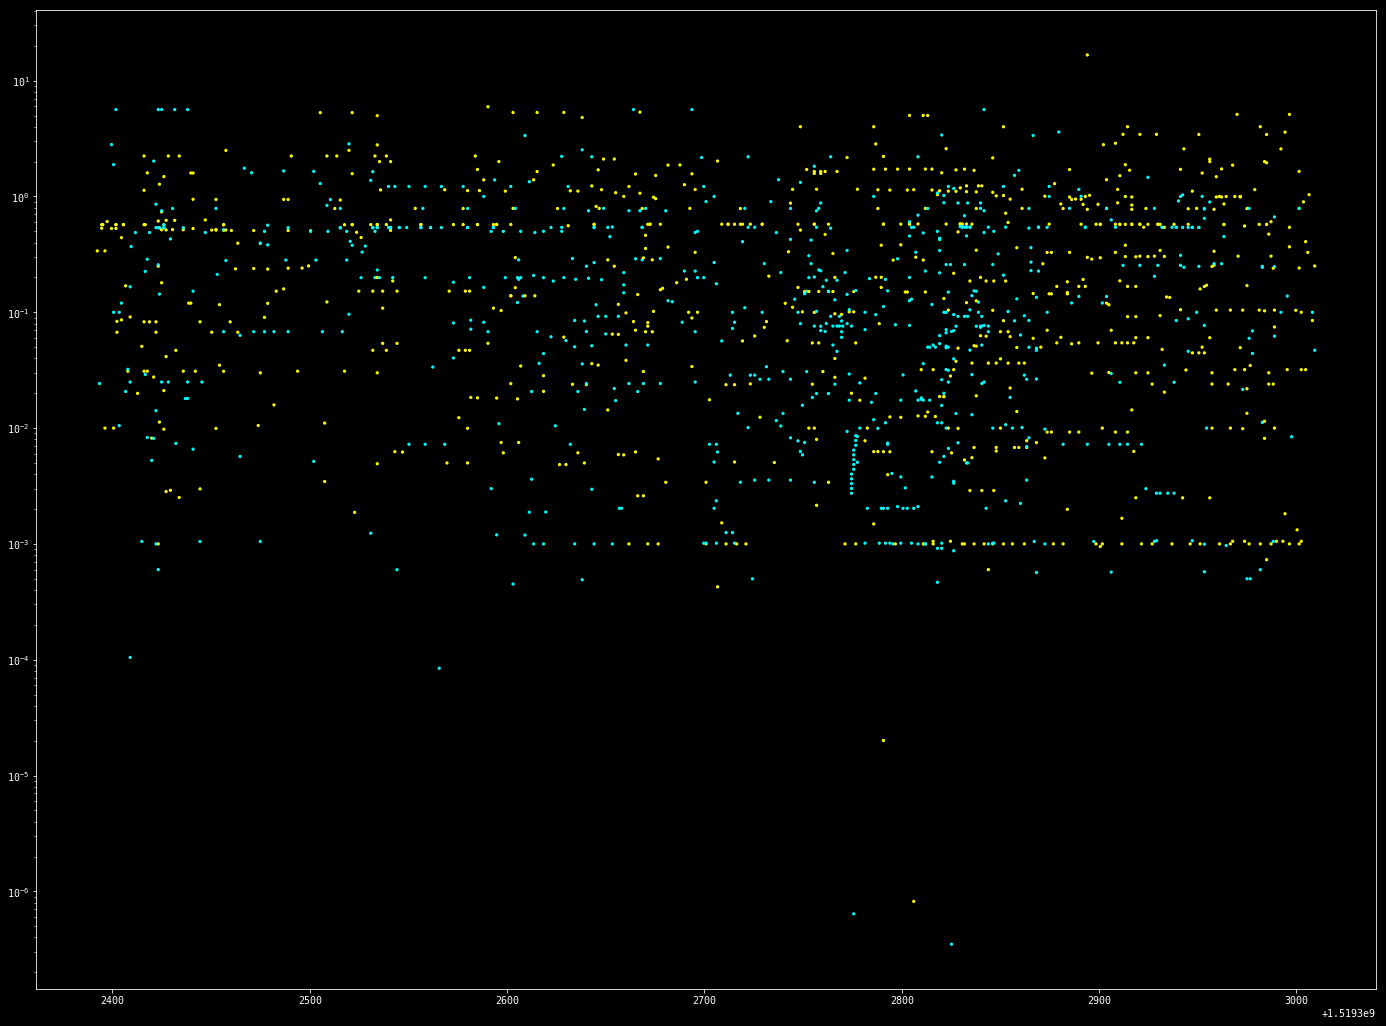
\includegraphics[width=14cm]{images/data-volmap-cancelled}
    }
    \caption{Volume map of cancelled bid and ask orders.}
    \label{fig:data-volmap-cancelled}
\end{figure}
\begin{figure}[H]
    \centering
    \makebox[\linewidth]{
        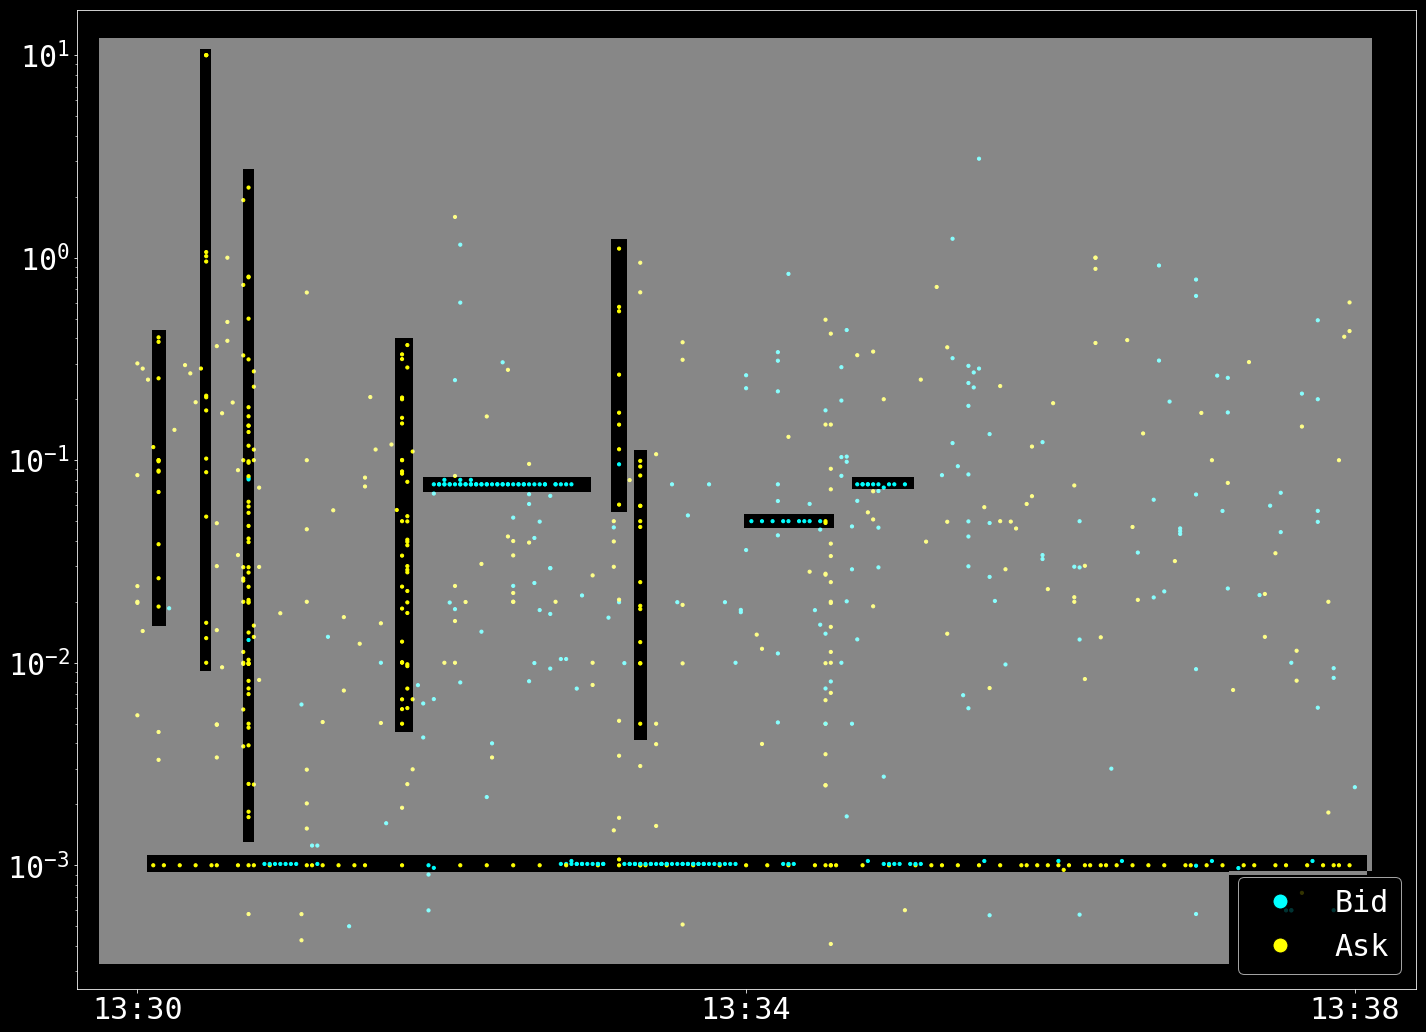
\includegraphics[width=14cm]{images/data-volmap-traded}
    }
    \caption{Volume map of trades initiated by a bid or ask order crossing the spread.}
    \label{fig:data-volmap-traded}
\end{figure}
Figure \ref{fig:data-volmap-crated} shows the volumes of the orders created.
The volumes of most of the orders placed were less than 1.0 BTC and significantly fewer orders had a larger volume, indicating that most of the participants were either willing to buy and sell only small quantities, or split their orders to minimize the market impact.
From a horizontal perspective, one can detect some orders on both sides, bids and asks, that were placed at the same time interval.
This behavior is particularly evident at the regions highlighted on the volume axis just below $10^0$.
This is likely to be one or multiple bots posting orders of the same volume and perhaps at different price levels.
Furthermore, a very distinctive diagonal-shaped pattern occurs when a trader posts orders of varying volumes within a short period of time.
This might be evidence of someone splitting a large order into small pieces (known as a buy- or sell wall).
Surprisingly, this behavior most often appeared both while and immediately after the market price started rising again. 

For at least some of the limit orders that did not result in a trade, the cancellation that followed was expected.
Figure \ref{fig:data-volmap-cancelled} shows the canceled orders over time.
Sequences of cancellations emerged more clearly when volumes were just below $10^0$ and at $10^{-3}$, and when these volumes and their respective time intervals correlated with the sequences of the orders created, as shown in Figure \ref{fig:data-volmap-crated} before.
Hence, it is likely that there was a trader following a strategy which involved creating and canceling orders in equal volumes.
A cancellation of one of the buy-walls that were created is particularly evident in both time stamps shortly after 13:34 and has a volume approximately equal to the one previously discovered during the observation of orders created.
That makes it likely that this wall was created and canceled by a single trader, and perhaps created again as the same pattern occurred again in the order-creation figure at a later time stamp.

So far, only posted limit orders or their cancellations were observed.
Not all of those limit orders might have resulted in a trade. Figure \ref{fig:data-volmap-traded} illustrates the volume map relating to the actual trades that occurred.
It is evident that the volumes of the trades transacted were $10^{-3}$, and oftentimes they had identical time intervals.
Additionally, a rapid series of many consecutive sales occurred around a time that correlates with the fall of the market price.
After the price fell, such sales were not present anymore.
Let us remember that there was one spike during the dip, and the time stamp related to it correlates strongly with the purchases (bids) visible in this figure before 13:34 with volumes of $10^{-1}$.
\\
\\
Various behavioral patterns were observed by investigating events initiated by market participants over time.
For some, their impact on the market price is immediately obvious; for others it is hard to interpret visually.
However, an attempt to find a correlation between the behavior of events and the resulting trades by means of learning techniques seems promising.
\\
\\
\textit{\textbf{Hypothesis:} patterns arising from events in which there were variations in the volumes posted determine future short-term trading behavior which can be exploited in favour of order placement.}

\subsection{Impact of traded price and volume}
\label{sec:data-hypthesis-trade-price-volume}

The price levels and volume of events over time was investigated in respect of each event type in the previous subsections.
Patterns were found and a hypothesis was proposed to the effect that the distribution of volumes of orders is an indicator of the future behavior of market participants. If true, the market price would eventually be influenced and this allows us to determine the optimal order placement.
The next logical step is to investigate the sum of the volumes traded over time, in combination with the price at which the asset was traded.
\begin{figure}[H]
    \centering
    \makebox[\linewidth]{
        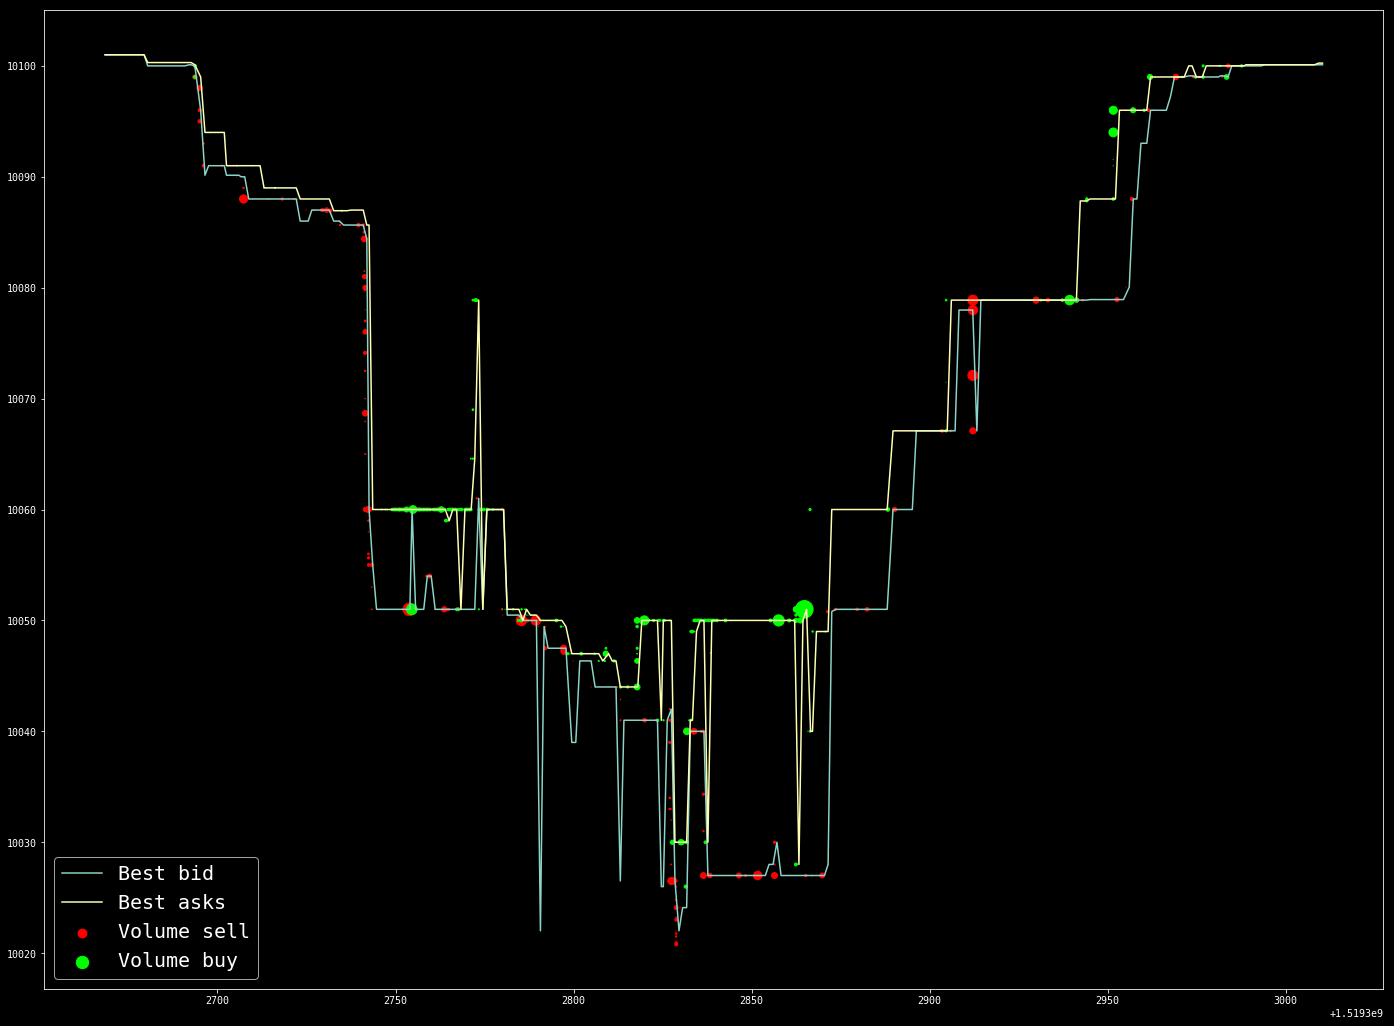
\includegraphics[width=14cm]{data-trade-volume}
    }
    \caption{Relation of trade volume to price movement.}
    \label{fig:data-trade-volume}
\end{figure}
Figure \ref{fig:data-trade-volume} shows the volumes of trades on both bid and ask sides which resulted in a buy or sell at a certain price.
The volumes of these trades are shown as dots of a size that indicates the traded volume and position of each dot defines its respective price.
As is known, a buy appears when one crosses the spread towards the seller side (ask) and a sell appears when crossing towards the buyer side (bid).
One can clearly see how buys are listed at the best ask price and sells are listed at the best bid level.
Before and during the dip, sells appeared consecutively, followed by one large sell transaction.
After that, a series of buy orders with low volumes occurred, and this  caused the minor spike.
Interestingly, a rather large buy trade appeared shortly before the price started to rise again.
Even though sell transactions took place in the middle of the price rise, participants continued buying shortly thereafter.
In conclusion, it is evident that a few trades with small volumes caused a certain noise in the overall trend.
Consecutive trades on one side or a single large trade, however, led the market price to move for a substantially longer period of time in one direction.
\\
\\
\textit{\textbf{Hypothesis:} consecutive small trades or one large trade give an impulse that drives the market price up or down.}


\section{Feature construction}
\label{sec:feature-engineering}
The previous section demonstrated certain trading behaviors of market participants in an order-driven market, which ultimately determines the development of the limit order book. 
Hypotheses were laid out which posit that the outcome in terms of a change in the order book constellation and price development can be related to the aforementioned trading behavior.
This suggests that orders can be placed and filled at limit levels which result in a favorable price.
The following subsections will introduce features that are derived from the previously collected (Section \ref{sec:data-collection}) and processed (Section \ref{sec:data-generation}) data and cover the assumptions stated in Section \ref{sec:data-hypotheses}.
Instead of manually extracting features such as those shown in \cite{nevmyvaka2006reinforcement, hwangdeep, fletcher2010multiple}, the aim of this project is to acquire knowledge directly from raw inputs, similar to a proven, successful method in the gaming sector\cite{mnih2013playing} and which was recently applied in the trading context\cite{lu2017agent}.

\subsection{Feature: price and size of historical orders}
\label{sec:data-feature-1}

The first feature represents the order book (as defined in Eq. \ref{eq:order-book}) and generated in Section \ref{sec:data-generation}.
More precisely, for each sample at time $t$, we use $n$ order book entries (Eq.\ref{eq:order-book-entry}) of $m$ of the order book states (Eq. \ref{eq:order-book-state}) with time stamp $ts \le t$.
As shown in Eq. \ref{eq:feature-bid-ask}, $s_{bidask} \in \mathbb{R^+}^{m\times2\times2n}$ is the state observed by a reinforcement learning agent.
The order book states are ordered such that $m$ is the closest to $t$.
The $n$ order book entries are closest to the spread in which only the price $bp$ (respectively $ap$) and size $bs$ (respectively $as$) are considered.

\begin{equation}\label{eq:feature-bid-ask}
s_{bidask} =\begin{bmatrix}
{\displaystyle \begin{pmatrix}
bp_{11} & bs_{11}\\
bp_{12} & bs_{12}\\
\vdots  & \vdots \\
bp_{1n} & bs_{1n}\\
ap_{11} & as_{11}\\
ap_{12} & as_{12}\\
\vdots  & \vdots \\
ap_{1n} & as_{1n}
\end{pmatrix}} & \begin{pmatrix}
bp_{21} & bs_{21}\\
bp_{22} & bs_{22}\\
\vdots  & \vdots \\
bp_{2n} & bs_{2n}\\
ap_{21} & as_{21}\\
ap_{22} & as_{22}\\
\vdots  & \vdots \\
ap_{2n} & as_{2n}
\end{pmatrix} & \cdots  & \begin{pmatrix}
bp_{m1} & bs_{m1}\\
bp_{m2} & bs_{m2}\\
\vdots  & \vdots \\
bp_{mn} & bs_{mn}\\
ap_{m1} & as_{m1}\\
ap_{m2} & as_{m2}\\
\vdots  & \vdots \\
ap_{mn} & as_{mn}
\end{pmatrix}
\end{bmatrix} \ 
\end{equation}

As the state will be observed by a deep learning agent that makes use of a neural network, the scaling of inputs will contribute to a faster learning process.
We therefore have applied normalization to the prices ($bp, ap$) with respect to the best ask price for each state, that is $ap_{i1}$.
Accordingly, we have also normalized the sizes ($bs, as$) by reference to the size provided at the best ask price $as_{i1}$.
While this method does not scale the values of prices and sizes within a predefined range, the values sill decrease significantly.
Furthermore, empirical observations show that the minimum and maximum prices within a single order book state do not differ by more than ~2\%, which determines the approximate scaling boundary.
\\
\\
This feature incorporates some of the previously stated hypotheses and therefore enables the learner to determine whether the statements are valid or not.
In particular, the feature includes historical order prices (hypothesis \ref{sec:data-hypthesis-order-price}), their volume (hypothesis \ref{sec:data-hypthesis-order-volume} and partly \ref{sec:data-hypthesis-order-trade-volume-time}).
\\
\\
\todo[inline]{Might be unnecessary according to our talk.}
There remain the questions of how large the window of $m$ order books states should be and the number of limit levels that $n$ should be chosen.
The following observation provides an insight into the parameters; however, by no means does it aim to make an estimate of how well the agent may perform under the consideration of a certain parameter setup.

In order to determine the impact of $n$ limit levels, we take the average of 100 evaluations whereas we take 1,000 random order book states for which we measure the Shannon entropy\cite{shannon2001mathematical} for a range of 40 limit levels (maximum of what goes from collection) on the bid and ask side, applied to price and size.
The entropy therefore serves as an indicator of how much information can be gained in respect of each limit level, derived from the change in price and size for each state.

\begin{figure}[H]
    \centering
    \begin{subfigure}[b]{0.45\textwidth}
        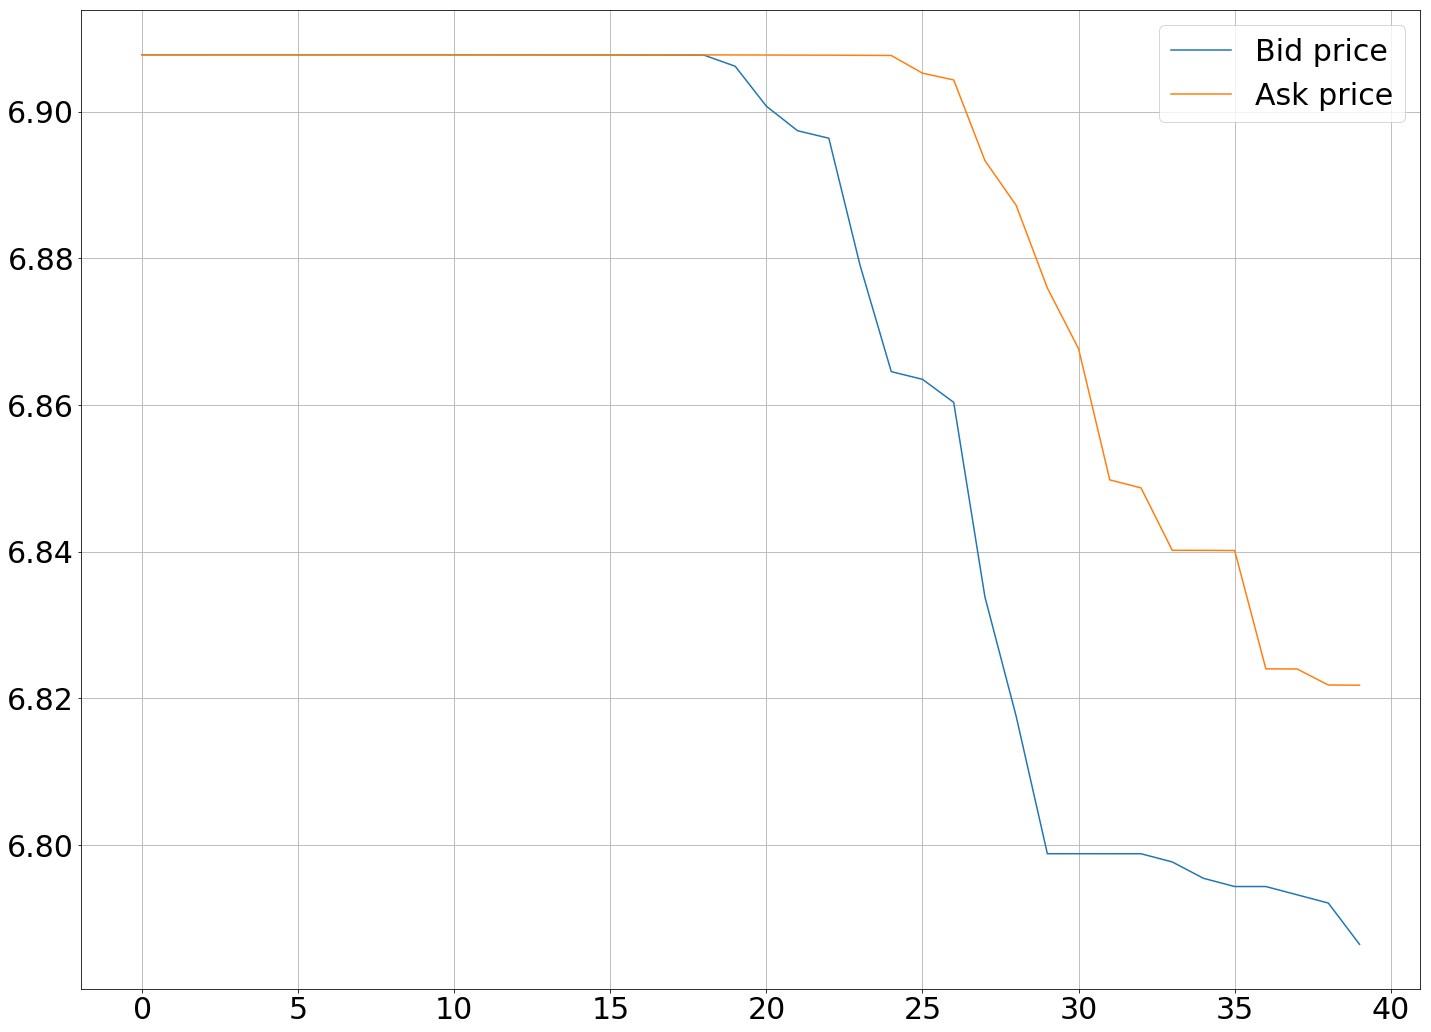
\includegraphics[width=\textwidth]{bidask-price-entropy}
        \caption{Entropy of order prices}
        \label{fig:bidask-price-entropy}
    \end{subfigure}
    \begin{subfigure}[b]{0.45\textwidth}
        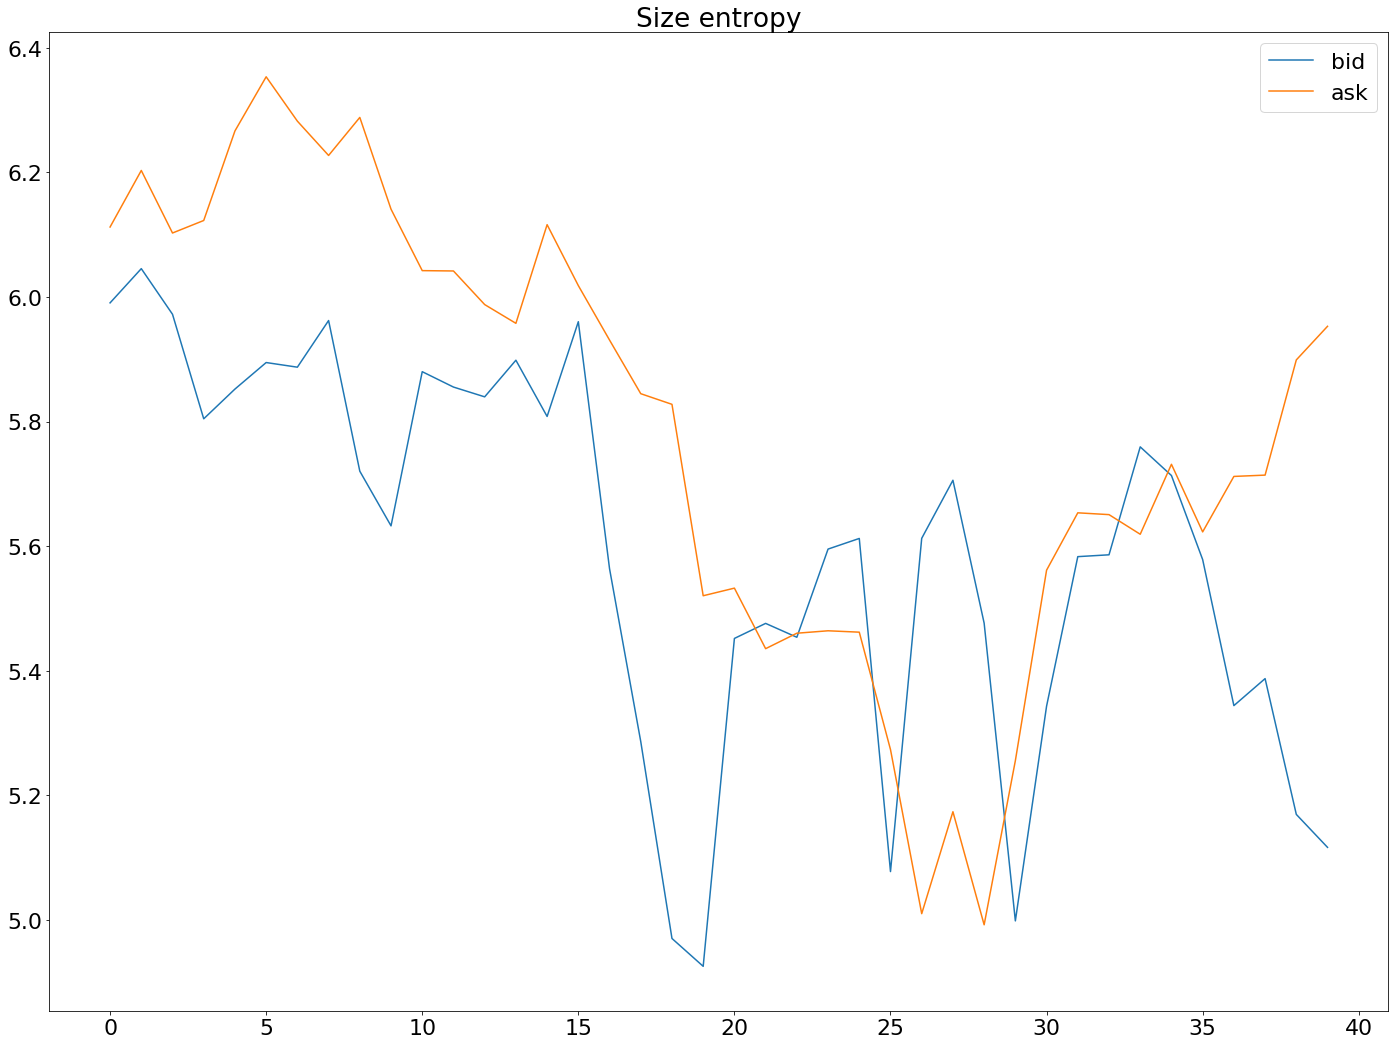
\includegraphics[width=\textwidth]{bidask-size-entropy}
        \caption{Entropy of order sizes}
        \label{fig:bidask-size-entropy}
    \end{subfigure}
    \caption{Entropy measured for 40 limit levels}\label{fig:bidask-entropy}
\end{figure}

It is noticeable that the entropy of prices of limit levels 0-30 on both bid and ask sides remains high, as shown in Figure \ref{fig:bidask-price-entropy}. 
The price becomes slightly more constant for limit levels $>30$. 
The entropy for order sizes, as shown in Figure \ref{fig:bidask-size-entropy}, drops after 20 limit levels, which indicates that the accumulated order size deep in the book is more constant. 
We therefore suggest considering at least 30 limit levels of the bid-ask feature.

\begin{figure}[H]
    \centering
    \begin{subfigure}[b]{0.45\textwidth}
        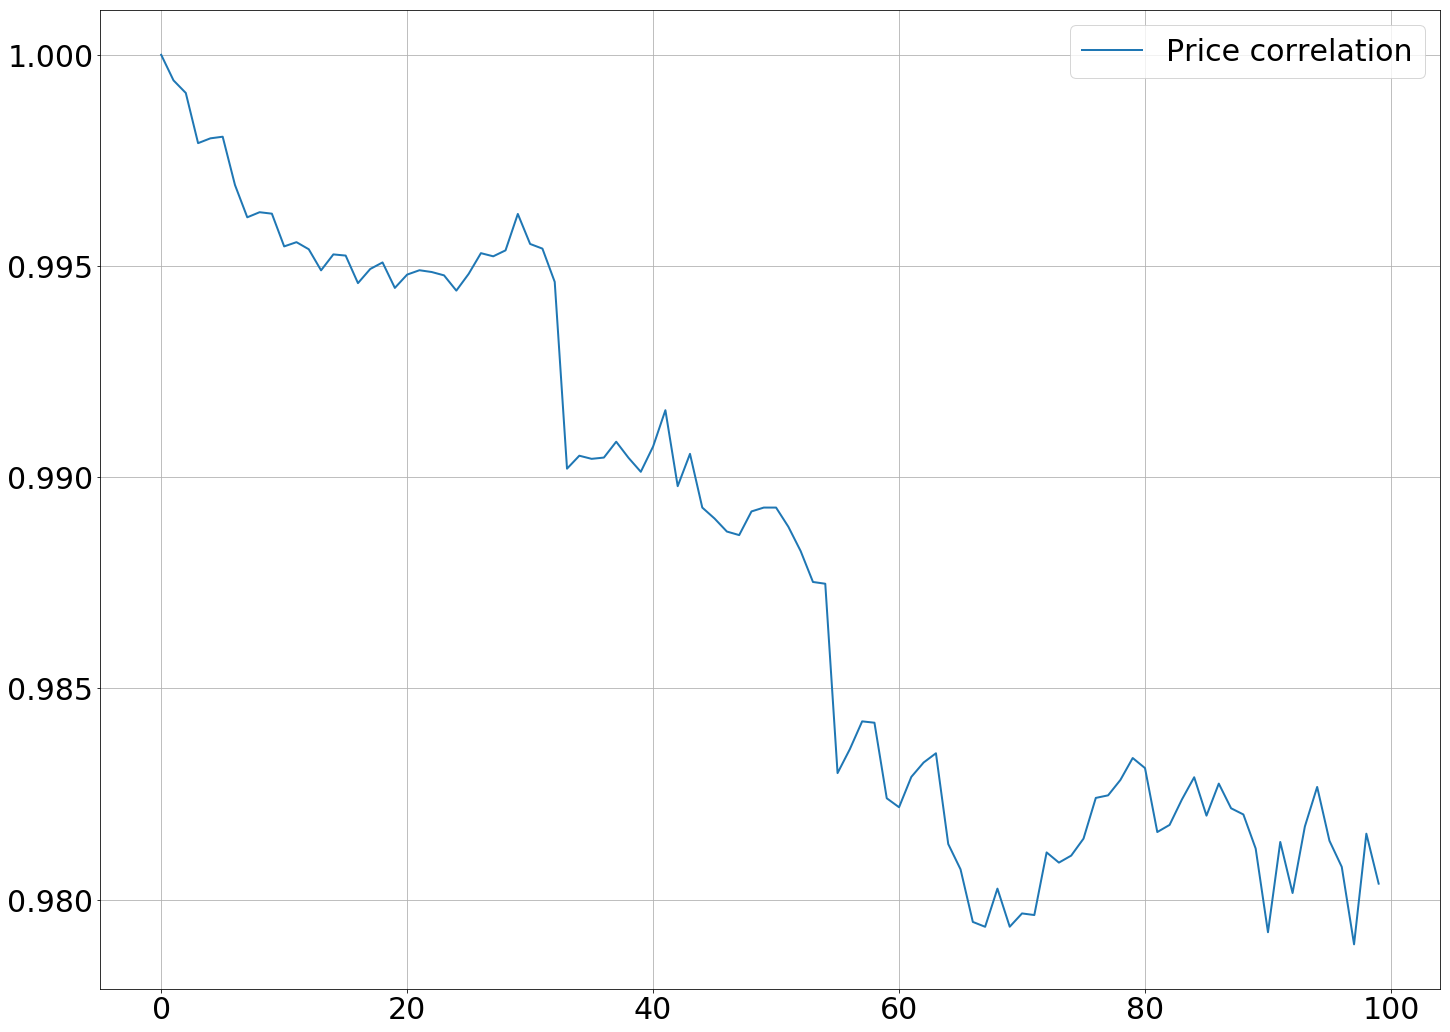
\includegraphics[width=\textwidth]{bidask-price-correlation}
        \caption{Correlation of order prices}
        \label{fig:bidask-price-correlation}
    \end{subfigure}
    \begin{subfigure}[b]{0.45\textwidth}
        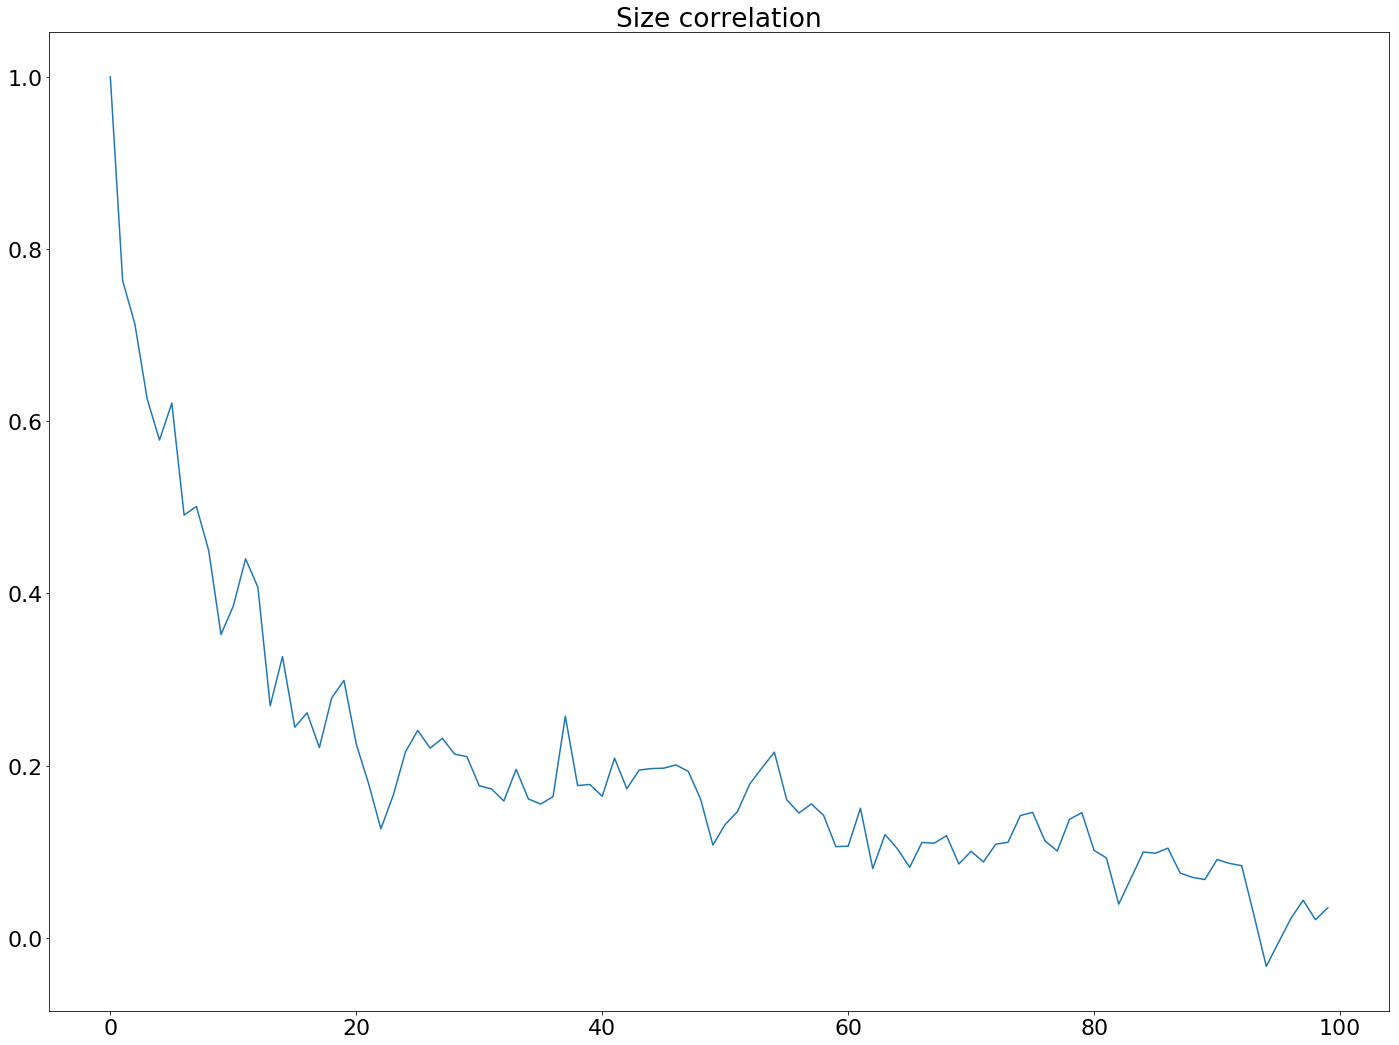
\includegraphics[width=\textwidth]{bidask-size-correlation}
        \caption{Correlation of order sizes}
        \label{fig:bidask-size-correlation}
    \end{subfigure}
    \caption{Correlation measured for 100 order book states}\label{fig:bidask-correlation}
\end{figure}

With this brief understanding of how limit levels $n$ affect order prices and sizes, we will try to make a statement about how order book states are related to the most recent state.
More precisely, we will determine the correlation between the order prices and sizes from the previous $m$ states and the most recent order book state.
We will take an average of 100 evaluations whereas we take a single order book state at time $t$ and a sequence of 100 previous order book states for each of which we measure the Shannon entropy\cite{shannon2001mathematical} to the state at $t$, whereas $n=40$ (maximum).
As can be seen in Figure \ref{fig:bidask-price-correlation}, the correlation of the price positions drop rapidly. However the effective change is not significant, indicating that the price changes are noticeable but overall do not differ much.
Order book states which lay more than 40 states in the past are slightly less correlated with the current state.
The correlation of order sizes, as shown in Figure \ref{fig:bidask-size-correlation} drops more rapidly and to a much greater extent than the order prices.
This indicates that traders choose a broad range of order sizes.
As a result, a window size of order book states $m$ greater than 40 states is suggested, in order to benefit from price differences within the feature.

\subsection{Feature: price and size of historical trades}
\label{sec:data-feature-2}
The previous feature provides information to the learner in order to reason about the hypotheses which are derived from orders placed and canceled.
In order to reason about whether or not trade events can provide a positive learning effect to the agent to optimize order placement, we construct a feature that covers the hypotheses \ref{sec:data-hypthesis-trade-price-volume} and partially \ref{sec:data-hypthesis-order-trade-volume-time}, as follows.
A $Trade$ (Eq. \ref{eq:trade}) carries an order side $os$, a quantity $q$ and a price $p$.
Similar to the previous feature, in this feature, we take $n$ trades into consideration, which occurred prior the time of the order placement.
More precisely, the feature is generated at some time $t$, when an order is placed, and therefore the time stamp $ts$ of the historical trades must satisfy $ts \leq t$.
\\
\\
A straightforward approach would be to construct the feature $s_{trade}$ as,
\begin{equation}
    s_{trade} =\begin{pmatrix}
        p_1 & q_1 & os_1 \\
        p_2 & q_2 & os_2 \\
        \vdots & \vdots & \vdots\\
        p_n & q_n & os_n \\
    \end{pmatrix}
    \ \forall \ p, q, os, ts \in Trade
\end{equation}, whereas $ts_n - ts_1 \leq m$.
However, trades do not occur at fixed time intervals and this causes the length of the vector to vary.
Accordingly, we calculate the time difference $\Delta{ts}$ between each historical trade and the subsequent historical trade.
For the most recent historical trade, the time difference is measured to the time of the order placement $t$.
That is,
\begin{equation}
    \Delta{ts}_i = \begin{cases}
    t - ts_i &\text{if i = 1}\\
    ts_{i+1} - ts_i &\text{otherwise}
    \end{cases}
\end{equation}

As a result we can redefine the feature $s_{trade}$, that is used by the learner as observation state, as,
\begin{equation}
    s_{trade} =\begin{pmatrix}
        \Delta{ts_1} & p_1 & q_1 & os_1 \\
        \Delta{ts_2} & p_2 & q_2 & os_2 \\
        \vdots & \vdots & \vdots & \vdots\\
        \Delta{ts_n} & p_n & q_n & os_n \\
    \end{pmatrix}
    \ \forall \ p, q, os, ts \in Trade
\end{equation}
\hfill
\\
\\
In addition, the new feature is normalized such that the prices are divided by the market price $p_t$ and the quantities are divided by the size of the order $q_t$ which is about to be placed at time $t$.
As a result, we constructed a feature vector of length $n$ (number of trades) that contains information about the price, order side and quantity of historical trades, as well as their order of occurrence.

\section{Conclusion}

Event data was collected from the Bittrex cryptocurrency exchange and a limit order book was reconstructed therefrom.
This limit order book serves as the historical data set and source for the match engine in order to simulate order placement. 
Subsequently the price chart, derived from the order book generated, was shown and the underlying event data were investigated.
Patterns were found which give insight into how market participants positioned their orders, with respect to price and size.
It was shown that the price movement was likely to be due to (1) an imbalance between bid and ask orders; (2) a distinctive way of posting or canceling orders; and (3) consecutive or impulsive trades.
These findings were incorporated within the two features constructed, and will serve as the observation state for the reinforcement learning agents that are described in the following chapter.